% ============================================================================
% CV5 RESULTS — NATIVE LaTeX tables under the unified 5-fold cross-validation
% protocol. The three \input fragments (cv5_{main,scaling,ablation}_table.tex) are
% regenerated from results_cv5/ by build_cv5_tex.py on every refresh cycle, and the
% paper is recompiled, so cells fill in real time as folds finish ("run..." = pending).
% They SUPERSEDE the pre-CV5 tables archived in archive/paper_pre_cv5_2026-07-13/.
% ============================================================================
\begin{table*}[t]
\centering
\IfFileExists{cv5_main_table.tex}{\setlength{\tabcolsep}{3pt}\renewcommand{\arraystretch}{1.5}
\resizebox{\textwidth}{!}{%
\begin{tabular}{l l c c c c c c c c c c c c c c c c c c}
\toprule
 & & & & & \multicolumn{8}{c}{Single-cell macro-F1 $\uparrow$} & \multicolumn{6}{c}{Multi-omics macro-F1 $\uparrow$} & \\
\cmidrule(lr){6-13}\cmidrule(lr){14-19}
Model & Type & $N_R$ & Param & FLOPs & Segerst. & Lung & Oesoph. & Baron & Muraro & T-cell & Spleen & Xin & Prostate & Bladder & Stomach & Pan-MC & Pan-Ex & Pan-3M & Avg \\
\midrule
Vanilla & -- & 4 & 300K & 1.00$\times$ & 62.5{\scriptsize$\pm$11.2} & 72.5{\scriptsize$\pm$2.5} & 58.7{\scriptsize$\pm$4.2} & 61.0{\scriptsize$\pm$8.5} & 80.2{\scriptsize$\pm$4.3} & 52.1{\scriptsize$\pm$3.5} & 48.3{\scriptsize$\pm$3.7} & 74.0{\scriptsize$\pm$12.1} & 66.8{\scriptsize$\pm$9.4} & 40.6{\scriptsize$\pm$5.8} & 44.5{\scriptsize$\pm$7.5} & 75.6{\scriptsize$\pm$3.5} & 94.2{\scriptsize$\pm$1.7} & 95.2{\scriptsize$\pm$1.5} & 66.2{\scriptsize$\pm$5.7} \\
\midrule
Recursive & -- & 2 & 75K & 0.50$\times$ & 65.8{\scriptsize$\pm$4.4} & 71.7{\scriptsize$\pm$2.8} & 57.3{\scriptsize$\pm$2.9} & 65.6{\scriptsize$\pm$2.8} & 79.8{\scriptsize$\pm$6.5} & 53.0{\scriptsize$\pm$2.0} & 48.8{\scriptsize$\pm$2.3} & 68.2{\scriptsize$\pm$2.4} & 66.2{\scriptsize$\pm$13.4} & 41.4{\scriptsize$\pm$1.3} & 46.0{\scriptsize$\pm$3.4} & 75.7{\scriptsize$\pm$2.9} & 94.6{\scriptsize$\pm$2.7} & 94.9{\scriptsize$\pm$1.5} & 66.4{\scriptsize$\pm$3.7} \\
 & -- & 3 & 75K & 0.75$\times$ & 64.5{\scriptsize$\pm$3.1} & 72.7{\scriptsize$\pm$2.0} & 57.5{\scriptsize$\pm$2.1} & 67.1{\scriptsize$\pm$8.7} & 78.7{\scriptsize$\pm$4.9} & 49.8{\scriptsize$\pm$4.4} & 49.4{\scriptsize$\pm$3.3} & 67.8{\scriptsize$\pm$7.3} & 63.2{\scriptsize$\pm$7.6} & 43.2{\scriptsize$\pm$6.2} & 45.7{\scriptsize$\pm$3.7} & 74.6{\scriptsize$\pm$2.7} & 94.4{\scriptsize$\pm$1.8} & 95.0{\scriptsize$\pm$1.4} & 66.0{\scriptsize$\pm$4.2} \\
 & -- & 4 & 75K & 1.00$\times$ & 61.4{\scriptsize$\pm$7.3} & 72.9{\scriptsize$\pm$2.9} & 56.9{\scriptsize$\pm$4.3} & 65.9{\scriptsize$\pm$2.7} & 75.8{\scriptsize$\pm$4.1} & 50.5{\scriptsize$\pm$3.5} & 49.4{\scriptsize$\pm$3.4} & 72.2{\scriptsize$\pm$5.2} & 65.3{\scriptsize$\pm$10.0} & 40.2{\scriptsize$\pm$1.1} & 43.2{\scriptsize$\pm$6.0} & 72.3{\scriptsize$\pm$1.8} & 96.3{\scriptsize$\pm$1.1} & 94.3{\scriptsize$\pm$1.1} & 65.5{\scriptsize$\pm$3.9} \\
\midrule
\textbf{MoR (general)} & Expert & 2 & 75K & 0.42$\times$ & 65.0{\scriptsize$\pm$6.2} & 72.9{\scriptsize$\pm$1.7} & 57.0{\scriptsize$\pm$3.5} & 58.0{\scriptsize$\pm$6.1} & 72.3{\scriptsize$\pm$2.9} & 50.6{\scriptsize$\pm$4.9} & 51.7{\scriptsize$\pm$1.4} & 68.0{\scriptsize$\pm$8.3} & 71.2{\scriptsize$\pm$11.8} & 39.7{\scriptsize$\pm$12.3} & 49.7{\scriptsize$\pm$6.3} & 77.7{\scriptsize$\pm$1.4} & 94.9{\scriptsize$\pm$1.7} & 94.6{\scriptsize$\pm$1.3} & 65.9{\scriptsize$\pm$5.0} \\
 & Expert & 3 & 75K & 0.59$\times$ & 60.7{\scriptsize$\pm$6.9} & 74.2{\scriptsize$\pm$1.7} & 58.4{\scriptsize$\pm$3.6} & 61.6{\scriptsize$\pm$2.3} & 69.3{\scriptsize$\pm$7.2} & 52.3{\scriptsize$\pm$2.4} & 47.5{\scriptsize$\pm$3.0} & 65.7{\scriptsize$\pm$7.5} & 63.4{\scriptsize$\pm$12.3} & 38.0{\scriptsize$\pm$8.0} & 42.3{\scriptsize$\pm$4.4} & 77.0{\scriptsize$\pm$1.1} & 96.4{\scriptsize$\pm$1.2} & 94.6{\scriptsize$\pm$1.6} & 64.4{\scriptsize$\pm$4.5} \\
 & Expert & 4 & 75K & 0.76$\times$ & 64.3{\scriptsize$\pm$11.6} & 72.3{\scriptsize$\pm$2.7} & 55.3{\scriptsize$\pm$2.6} & 68.9{\scriptsize$\pm$3.7} & 74.8{\scriptsize$\pm$4.7} & 50.9{\scriptsize$\pm$4.7} & 53.2{\scriptsize$\pm$1.3} & 66.1{\scriptsize$\pm$9.7} & 62.8{\scriptsize$\pm$10.1} & 43.7{\scriptsize$\pm$2.8} & 45.2{\scriptsize$\pm$4.1} & 75.5{\scriptsize$\pm$3.0} & 94.3{\scriptsize$\pm$2.0} & 94.3{\scriptsize$\pm$1.3} & 65.8{\scriptsize$\pm$4.6} \\
 & Token & 2 & 75K & 0.42$\times$ & 57.4{\scriptsize$\pm$6.6} & 72.2{\scriptsize$\pm$2.7} & 57.7{\scriptsize$\pm$1.8} & 66.2{\scriptsize$\pm$8.5} & 82.5{\scriptsize$\pm$7.1} & 50.7{\scriptsize$\pm$2.2} & 50.6{\scriptsize$\pm$2.5} & 68.9{\scriptsize$\pm$6.0} & 76.2{\scriptsize$\pm$3.8} & 35.7{\scriptsize$\pm$7.8} & 47.7{\scriptsize$\pm$4.0} & 76.4{\scriptsize$\pm$4.6} & 95.8{\scriptsize$\pm$1.1} & 94.3{\scriptsize$\pm$2.8} & 66.6{\scriptsize$\pm$4.4} \\
 & Token & 3 & 75K & 0.52$\times$ & 55.1{\scriptsize$\pm$5.0} & 70.5{\scriptsize$\pm$3.3} & 56.6{\scriptsize$\pm$3.4} & 64.0{\scriptsize$\pm$4.6} & 75.9{\scriptsize$\pm$4.7} & 55.8{\scriptsize$\pm$3.0} & 49.2{\scriptsize$\pm$2.1} & 70.1{\scriptsize$\pm$3.5} & 70.9{\scriptsize$\pm$11.7} & 41.3{\scriptsize$\pm$8.6} & 46.5{\scriptsize$\pm$4.5} & 77.2{\scriptsize$\pm$3.9} & 91.9{\scriptsize$\pm$2.4} & 93.6{\scriptsize$\pm$2.1} & 65.6{\scriptsize$\pm$4.5} \\
 & Token & 4 & 75K & 0.56$\times$ & 60.7{\scriptsize$\pm$5.8} & 73.3{\scriptsize$\pm$2.4} & 59.8{\scriptsize$\pm$3.7} & 65.2{\scriptsize$\pm$5.5} & 81.6{\scriptsize$\pm$2.7} & 50.4{\scriptsize$\pm$2.2} & 51.1{\scriptsize$\pm$3.1} & 62.3{\scriptsize$\pm$5.7} & \cellcolor{bestgreen}\textbf{78.5{\scriptsize$\pm$3.1}} & 40.6{\scriptsize$\pm$6.9} & 48.8{\scriptsize$\pm$3.6} & 78.0{\scriptsize$\pm$4.6} & 94.6{\scriptsize$\pm$1.7} & 95.3{\scriptsize$\pm$1.6} & 67.1{\scriptsize$\pm$3.8} \\
\midrule
\textbf{bioMoR (ERA)} & Expert & 2 & 75K & 0.42$\times$ & 72.4{\scriptsize$\pm$2.9} & \cellcolor{bestgreen}\textbf{80.3{\scriptsize$\pm$1.5}} & 71.0{\scriptsize$\pm$1.5} & \cellcolor{bestgreen}\textbf{85.2{\scriptsize$\pm$2.9}} & 83.8{\scriptsize$\pm$3.1} & 69.2{\scriptsize$\pm$0.7} & 60.3{\scriptsize$\pm$1.9} & 76.3{\scriptsize$\pm$9.6} & 55.6{\scriptsize$\pm$4.6} & 28.2{\scriptsize$\pm$4.5} & 43.6{\scriptsize$\pm$3.9} & 85.5{\scriptsize$\pm$1.9} & 97.6{\scriptsize$\pm$0.6} & 96.0{\scriptsize$\pm$1.3} & 71.8{\scriptsize$\pm$2.9} \\
 & Expert & 3 & 75K & 0.59$\times$ & \cellcolor{bestgreen}\textbf{76.1{\scriptsize$\pm$2.9}} & 80.1{\scriptsize$\pm$0.3} & 69.2{\scriptsize$\pm$1.6} & 81.6{\scriptsize$\pm$2.7} & \cellcolor{bestgreen}\textbf{85.1{\scriptsize$\pm$7.6}} & 69.6{\scriptsize$\pm$0.6} & \cellcolor{bestgreen}\textbf{61.4{\scriptsize$\pm$1.7}} & \cellcolor{bestgreen}\textbf{80.1{\scriptsize$\pm$7.0}} & 58.7{\scriptsize$\pm$6.2} & 34.2{\scriptsize$\pm$6.5} & 49.2{\scriptsize$\pm$5.0} & 86.0{\scriptsize$\pm$1.0} & 96.9{\scriptsize$\pm$0.6} & 96.3{\scriptsize$\pm$0.8} & 73.2{\scriptsize$\pm$3.2} \\
 & Expert & 4 & 75K & 0.76$\times$ & 72.2{\scriptsize$\pm$4.5} & 80.0{\scriptsize$\pm$1.2} & 70.8{\scriptsize$\pm$1.6} & 81.9{\scriptsize$\pm$1.9} & 83.7{\scriptsize$\pm$4.9} & \cellcolor{bestgreen}\textbf{70.0{\scriptsize$\pm$1.9}} & 59.7{\scriptsize$\pm$0.8} & 72.7{\scriptsize$\pm$5.5} & 56.2{\scriptsize$\pm$7.2} & \cellcolor{bestgreen}\textbf{47.1{\scriptsize$\pm$7.1}} & 46.0{\scriptsize$\pm$2.6} & 85.8{\scriptsize$\pm$1.5} & \cellcolor{bestgreen}\textbf{97.8{\scriptsize$\pm$0.4}} & \cellcolor{bestgreen}\textbf{98.0{\scriptsize$\pm$0.4}} & 73.0{\scriptsize$\pm$3.0} \\
\textbf{\quad + Token ($N_R{=}2$)} & Token & 2 & 75K & 0.42$\times$ & 74.4{\scriptsize$\pm$6.8} & 79.4{\scriptsize$\pm$1.3} & \cellcolor{bestgreen}\textbf{71.1{\scriptsize$\pm$2.4}} & 82.9{\scriptsize$\pm$5.0} & 83.8{\scriptsize$\pm$3.2} & 68.6{\scriptsize$\pm$1.7} & 60.3{\scriptsize$\pm$1.2} & 69.1{\scriptsize$\pm$6.6} & 56.4{\scriptsize$\pm$2.7} & 45.0{\scriptsize$\pm$13.8} & 44.2{\scriptsize$\pm$3.5} & 85.1{\scriptsize$\pm$1.5} & 96.6{\scriptsize$\pm$1.6} & 95.5{\scriptsize$\pm$2.2} & 72.3{\scriptsize$\pm$3.8} \\
\textbf{\quad + Token ($N_R{=}3$)} & Token & 3 & 75K & 0.52$\times$ & 73.6{\scriptsize$\pm$7.0} & 80.2{\scriptsize$\pm$1.5} & 71.0{\scriptsize$\pm$1.2} & 83.9{\scriptsize$\pm$3.0} & 78.4{\scriptsize$\pm$4.8} & 68.6{\scriptsize$\pm$0.9} & 61.0{\scriptsize$\pm$1.0} & 77.2{\scriptsize$\pm$5.3} & 60.9{\scriptsize$\pm$6.0} & 39.6{\scriptsize$\pm$13.7} & 45.4{\scriptsize$\pm$4.8} & 84.8{\scriptsize$\pm$2.3} & 96.7{\scriptsize$\pm$1.5} & 95.8{\scriptsize$\pm$1.0} & 72.6{\scriptsize$\pm$3.9} \\
\textbf{\quad + Token choice} & Token & 4 & 75K & 0.56$\times$ & 75.8{\scriptsize$\pm$2.8} & 79.7{\scriptsize$\pm$0.9} & 70.8{\scriptsize$\pm$2.1} & 82.9{\scriptsize$\pm$4.0} & 81.9{\scriptsize$\pm$6.8} & 69.8{\scriptsize$\pm$1.2} & 61.0{\scriptsize$\pm$0.6} & 76.1{\scriptsize$\pm$8.9} & 60.2{\scriptsize$\pm$1.2} & 39.5{\scriptsize$\pm$5.9} & \cellcolor{bestgreen}\textbf{51.4{\scriptsize$\pm$5.0}} & \cellcolor{bestgreen}\textbf{86.0{\scriptsize$\pm$1.9}} & 97.2{\scriptsize$\pm$0.6} & 96.4{\scriptsize$\pm$1.6} & 73.5{\scriptsize$\pm$3.1} \\
\bottomrule
\end{tabular}}
}{\emph{(main-results table renders here as 5-fold CV runs land)}}
\caption{\textbf{Main results: the efficiency ladder (5-fold CV).} Macro-F1 mean$\pm$SD;
\textbf{bold} = best per column; Avg over the $11$ core datasets (PM/PC/3M shown separately,
not averaged). The learned graph supplies the accuracy gain at $4\times$ fewer parameters.}
\label{tab:main_cv5}\label{tab:learned}\label{tab:ladder}
\end{table*}

% NEW Table 3 -- the injection-site ablation is our main contribution: WHERE the
% biological interaction should enter. (The former PATH-comparable positive-class F1
% table has been moved to the supplementary.)
\begin{table}[t]
\centering
\IfFileExists{cv5_injection_table.tex}{\resizebox{\columnwidth}{!}{%
\begin{tabular}{lcccc}
\toprule
Dataset & None & Router only & Embedding only & Both (bioMoR) \\
\midrule
\multicolumn{5}{l}{\emph{Single-cell (co-expression graph)}}\\
Baron & 63.6{\scriptsize$\pm$8.8} & 66.6{\scriptsize$\pm$3.1} & 79.1{\scriptsize$\pm$4.9} & \textbf{81.3{\scriptsize$\pm$4.9}} \\
Muraro & 76.8{\scriptsize$\pm$8.9} & 76.9{\scriptsize$\pm$6.3} & 87.0{\scriptsize$\pm$4.8} & \textbf{87.3{\scriptsize$\pm$4.4}} \\
\midrule
\multicolumn{5}{l}{\emph{Multi-omics (provided Reactome pathway graph)}}\\
PM & 81.0{\scriptsize$\pm$3.1} & 81.0{\scriptsize$\pm$2.3} & 85.9{\scriptsize$\pm$2.3} & \textbf{86.8{\scriptsize$\pm$1.7}} \\
3M & 94.5{\scriptsize$\pm$1.4} & 95.6{\scriptsize$\pm$0.9} & 95.5{\scriptsize$\pm$1.0} & \textbf{95.9{\scriptsize$\pm$1.8}} \\
\midrule
\textbf{Avg} & 79.0{\scriptsize$\pm$11.0} & 80.0{\scriptsize$\pm$10.4} & 86.9{\scriptsize$\pm$5.8} & \textbf{87.8{\scriptsize$\pm$5.2}} \\
\bottomrule
\end{tabular}
}
}{\emph{(injection-site ablation table renders here as runs land)}}
\caption{\textbf{Where should biology enter? (main contribution).} The interaction graph
injected at the embedding, the router (zero-init graph-conv), or both, under 5-fold CV.
\emph{Both} is the winning site on every cohort shown---defining bioMoR.}
\label{tab:injection}
\end{table}

\begin{figure}[t]
\centering
\IfFileExists{figs/biorouter_bars.pdf}{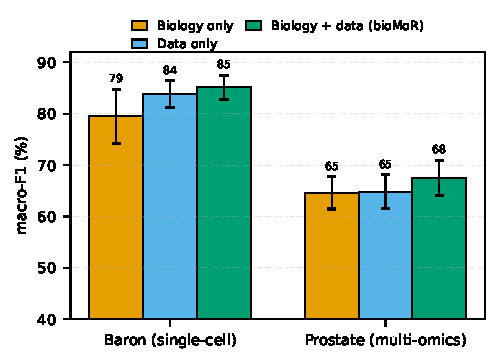
\includegraphics[width=\columnwidth]{figs/biorouter_bars.pdf}}{\emph{(bio-router ablation bar chart renders here)}}
\caption{\textbf{Biology in the router.} Depth-router ablation (5-fold CV) on Baron and
Prostate: fixed biology-only, data-only learned, and their combination. The learned graph
matches or beats fixed; combining is best---biology helps only when learned, not imposed.}
\label{fig:biorouter}
\end{figure}

\begin{figure}[t]
\centering
\IfFileExists{figs/baron_loss.pdf}{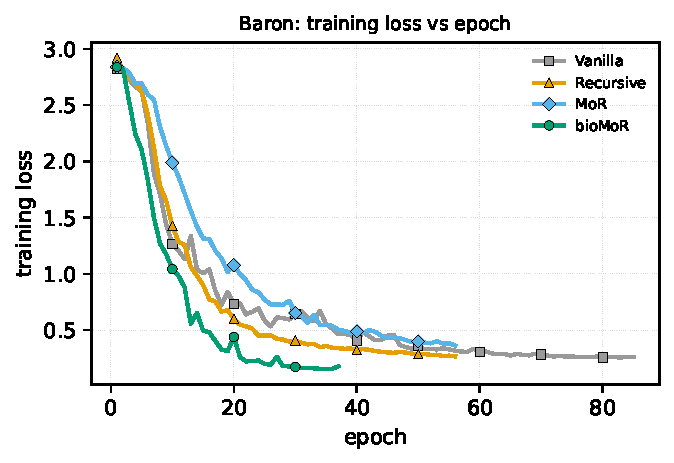
\includegraphics[width=0.49\columnwidth]{figs/baron_loss.pdf}}{}%
\hfill
\IfFileExists{figs/baron_val_f1.pdf}{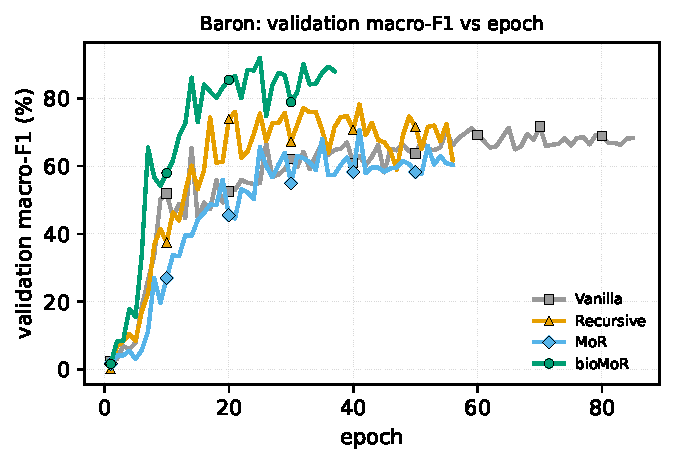
\includegraphics[width=0.49\columnwidth]{figs/baron_val_f1.pdf}}{}%
\caption{\textbf{Training dynamics on Baron.} Training loss (left) and validation macro-F1
(right) vs.\ epoch, learned-graph $K{=}4$ on fold~0 of the shared 5-fold split.}
\label{fig:baron_curves}
\end{figure}

\begin{figure}[t]
\centering
\IfFileExists{figs/pareto_efficiency.pdf}{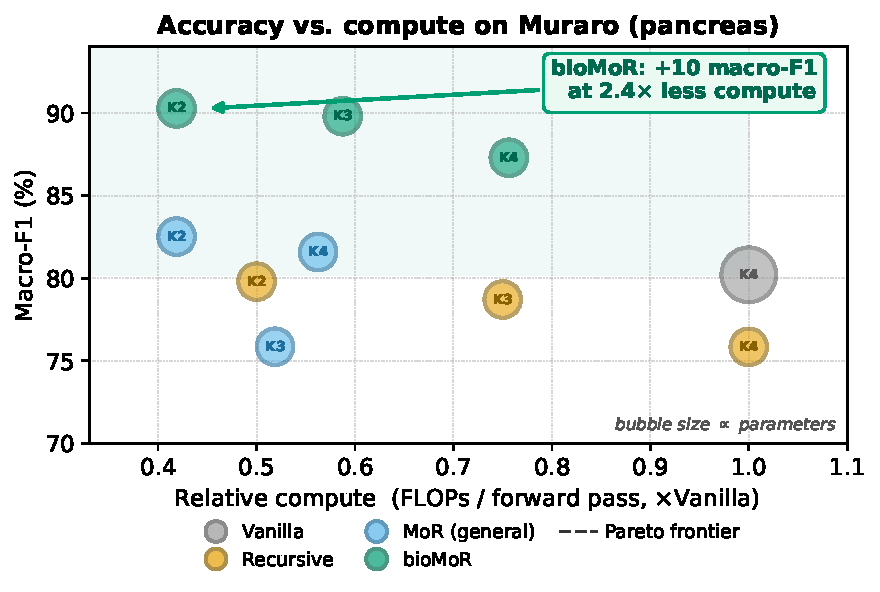
\includegraphics[width=\columnwidth]{figs/pareto_efficiency.pdf}}{\emph{(accuracy-vs-compute Pareto figure renders here as runs land)}}
\caption{\textbf{Accuracy--compute trade-off on Baron.} Macro-F1 vs.\ relative FLOPs
(norm.\ to Vanilla); marker size $\propto$ parameters. bioMoR is on the Pareto frontier;
the Vanilla stack ($4\times$ parameters, full compute) is dominated.}
\label{fig:pareto}
\end{figure}

% Model-size scaling table (tab:scaling / fig:scaling_cv5) moved to the supplementary.

\begin{table}[t]
\centering
\IfFileExists{cv5_ablation_table.tex}{\resizebox{\columnwidth}{!}{%
\begin{tabular}{l cc cc}
\toprule
Condition & SC macro-F1 & $\Delta$SC & MO macro-F1 & $\Delta$MO \\
\midrule
\addlinespace[1pt]\multicolumn{5}{l}{\textbf{1. Biological interaction graph}}\\
\emph{bioMoR learned (baseline)} & \textbf{74.0{\scriptsize$\pm$2.8}} &  & \textbf{54.9{\scriptsize$\pm$6.5}} &  \\
\quad none (no graph) & 62.7{\scriptsize$\pm$5.2} & \textcolor[HTML]{B00020}{-11.3} & 52.2{\scriptsize$\pm$3.1} & \textcolor[HTML]{B00020}{-2.6} \\
\quad coexpr / curated (fixed) & 50.0{\scriptsize$\pm$6.5} & \textcolor[HTML]{B00020}{-24.0} & 52.6{\scriptsize$\pm$5.0} & \textcolor[HTML]{B00020}{-2.2} \\
\quad random (deg.-matched) & 62.2{\scriptsize$\pm$3.8} & \textcolor[HTML]{B00020}{-11.8} & 54.1{\scriptsize$\pm$5.9} & \textcolor[HTML]{B00020}{-0.8} \\
\quad warm-start from curated & 74.6{\scriptsize$\pm$3.8} & \textcolor[HTML]{1A7F37}{+0.6} & -- & -- \\
\quad fuse coexpr graph & 76.1{\scriptsize$\pm$3.2} & \textcolor[HTML]{1A7F37}{+2.1} & -- & -- \\
\quad fuse RANDOM (control) & 73.5{\scriptsize$\pm$3.3} & \textcolor[HTML]{B00020}{-0.5} & -- & -- \\
\addlinespace[1pt]\multicolumn{5}{l}{\textbf{2. Recursion \& routing (MoR-general)}}\\
\emph{$N_R{=}4$, $M{=}128$ shared (baseline)} & \textbf{63.2{\scriptsize$\pm$5.1}} &  & -- &  \\
\quad share: sequence & 63.9{\scriptsize$\pm$5.2} & \textcolor[HTML]{1A7F37}{+0.6} & -- & -- \\
\quad share: middle-cycle & 63.5{\scriptsize$\pm$5.1} & \textcolor[HTML]{1A7F37}{+0.2} & -- & -- \\
\quad share: middle-seq. & 62.4{\scriptsize$\pm$5.3} & \textcolor[HTML]{B00020}{-0.9} & -- & -- \\
\quad router: MLP & 63.5{\scriptsize$\pm$4.2} & \textcolor[HTML]{1A7F37}{+0.3} & -- & -- \\
\quad no load-balance loss & 63.6{\scriptsize$\pm$4.6} & \textcolor[HTML]{1A7F37}{+0.4} & -- & -- \\
\quad markers: random & 65.3{\scriptsize$\pm$4.0} & \textcolor[HTML]{1A7F37}{+2.1} & -- & -- \\
\quad markers: variance & 67.3{\scriptsize$\pm$3.9} & \textcolor[HTML]{1A7F37}{+4.1} & -- & -- \\
\quad budget $M{=}64$ & 53.7{\scriptsize$\pm$5.6} & \textcolor[HTML]{B00020}{-9.6} & -- & -- \\
\quad budget $M{=}256$ & 71.2{\scriptsize$\pm$4.3} & \textcolor[HTML]{1A7F37}{+7.9} & -- & -- \\
\quad $N_R{=}1$ (no recursion) & 60.2{\scriptsize$\pm$5.2} & \textcolor[HTML]{B00020}{-3.0} & -- & -- \\
\quad $N_R{=}6$ & 63.1{\scriptsize$\pm$4.9} & \textcolor[HTML]{B00020}{-0.1} & -- & -- \\
\quad $N_R{=}8$ & 62.7{\scriptsize$\pm$4.9} & \textcolor[HTML]{B00020}{-0.5} & -- & -- \\
\addlinespace[1pt]\multicolumn{5}{l}{\textbf{3. Input modality (multi-omics)}}\\
\emph{mut+CNV (baseline)} & -- &  & \textbf{50.6{\scriptsize$\pm$5.7}} &  \\
\quad CNV only & -- & -- & 56.0{\scriptsize$\pm$4.7} & \textcolor[HTML]{1A7F37}{+5.4} \\
\quad mutation only & -- & -- & 47.3{\scriptsize$\pm$6.7} & \textcolor[HTML]{B00020}{-3.3} \\
\bottomrule
\end{tabular}}
}{\emph{(ablation table renders here as runs land)}}
\caption{\textbf{Component ablations.} Three families---biological interaction graph,
recursion \& routing, and input modality. SC/MO = mean macro-F1 over the $8$ SC and $3$
P-NET suites; $\Delta$ vs.\ the italic family baseline (green $+$, red $-$).}
\label{tab:ablation_cv5}\label{tab:confound}
\end{table}
